\documentclass{beamer}

% Theme choice
\usetheme{Madrid} % You can change to e.g., Warsaw, Berlin, CambridgeUS, etc.

% Encoding and font
\usepackage[utf8]{inputenc}
\usepackage[T1]{fontenc}

% Graphics and tables
\usepackage{graphicx}
\usepackage{booktabs}

% Code listings
\usepackage{listings}
\lstset{
basicstyle=\ttfamily\small,
keywordstyle=\color{blue},
commentstyle=\color{gray},
stringstyle=\color{red},
breaklines=true,
frame=single
}

% Math packages
\usepackage{amsmath}
\usepackage{amssymb}

% Colors
\usepackage{xcolor}

% TikZ and PGFPlots
\usepackage{tikz}
\usepackage{pgfplots}
\pgfplotsset{compat=1.18}
\usetikzlibrary{positioning}

% Hyperlinks
\usepackage{hyperref}

% Title information
\title{Implementing Cryptography in Python}
\author{Your Name}
\institute{Your Institution}
\date{\today}

\begin{document}

\frame{\titlepage}

\begin{frame}[fragile]
    \frametitle{Introduction to Cryptography in Python}
    \begin{block}{Overview of Cryptography}
        \begin{itemize}
            \item \textbf{Definition}: The science of securing information and ensuring privacy through encoding and decoding messages.
            \item \textbf{Purpose}: Protects data integrity, confidentiality, and authenticity in applications such as online banking, messaging apps, and secure communications.
        \end{itemize}
    \end{block}
\end{frame}

\begin{frame}[fragile]
    \frametitle{Role of Cryptography in Data Security}
    \begin{itemize}
        \item \textbf{Confidentiality}: Protects sensitive information from unauthorized access.
        \begin{itemize}
            \item \textit{Example}: Using encryption for emails ensures that only the intended recipient can read the content.
        \end{itemize}
        
        \item \textbf{Integrity}: Assures data has not been altered.
        \begin{itemize}
            \item \textit{Example}: Adding hash functions detects changes to files.
        \end{itemize}
        
        \item \textbf{Authentication}: Verifies identity of users/systems.
        \begin{itemize}
            \item \textit{Example}: Digital signatures confirm that a message is from a legitimate source.
        \end{itemize}
        
        \item \textbf{Non-repudiation}: Prevents denial of commitments, essential for legal accountability in transactions.
    \end{itemize}
\end{frame}

\begin{frame}[fragile]
    \frametitle{Why Python for Cryptographic Implementations?}
    \begin{itemize}
        \item \textbf{Ease of Use}: Python’s simple syntax is ideal for beginners and experienced developers.
        \item \textbf{Rich Libraries}: Libraries like \texttt{cryptography}, \texttt{PyCrypto}, and \texttt{hashlib} provide robust cryptographic tools.
        \item \textbf{Community Support}: Extensive documentation and a strong community facilitate learning and troubleshooting.
        \item \textbf{Cross-Platform Compatibility}: Python works across multiple systems, ensuring broad application of cryptographic solutions.
    \end{itemize}
\end{frame}

\begin{frame}[fragile]
    \frametitle{Example of Hashing in Python}
    \begin{lstlisting}[language=Python]
import hashlib

message = "Secure Data"
hashed_message = hashlib.sha256(message.encode()).hexdigest()
print("Hashed Message:", hashed_message)
    \end{lstlisting}
\end{frame}

\begin{frame}[fragile]
    \frametitle{Key Points to Emphasize}
    \begin{itemize}
        \item Cryptography is essential for securing sensitive data in our digital lives.
        \item Python's simplicity and powerful libraries make it an ideal choice for cryptographic methods.
        \item Learning cryptography through Python allows developers to protect user data and enhance cybersecurity.
    \end{itemize}
\end{frame}

\begin{frame}
    \frametitle{Learning Objectives}
    In this chapter, we will explore the practical implementation of cryptographic algorithms using Python. 
    Understanding these objectives will equip you with the knowledge and skills necessary to integrate cryptography into your applications effectively.
\end{frame}

\begin{frame}
    \frametitle{Learning Objectives - Key Concepts}
    \begin{enumerate}
        \item \textbf{Understand the Basics of Cryptography}
        \begin{itemize}
            \item Grasp key concepts including symmetric and asymmetric encryption, hashing, and digital signatures.
            \item Example: Differentiate between symmetric encryption (e.g., AES) and asymmetric encryption (e.g., RSA).
        \end{itemize}
        
        \item \textbf{Explore Python Libraries for Cryptography}
        \begin{itemize}
            \item Familiarize yourself with libraries like \textbf{PyCryptodome}, \textbf{cryptography}, and \textbf{hashlib}.
            \item Example: Generate a hash using hashlib.
        \end{itemize}
    \end{enumerate}
\end{frame}

\begin{frame}[fragile]
    \frametitle{Example: Generating a Hash}
    \begin{lstlisting}[language=Python]
    import hashlib
    message = "Hello, World!"
    hash_object = hashlib.sha256(message.encode())
    hex_dig = hash_object.hexdigest()
    print(hex_dig)  # Output will be the SHA-256 hash of "Hello, World!"
    \end{lstlisting}
\end{frame}

\begin{frame}
    \frametitle{Learning Objectives - Implementation}
    \begin{enumerate}
        \setcounter{enumi}{2}
        \item \textbf{Implement Key Management Practices}
        \begin{itemize}
            \item Understand secure key management: key generation, storage, and rotation.
        \end{itemize}
        
        \item \textbf{Learn to Encrypt and Decrypt Data}
        \begin{itemize}
            \item Implement data encryption and decryption techniques in Python.
            \item Example: Encrypting a message using the cryptography library.
        \end{itemize}
    \end{enumerate}
\end{frame}

\begin{frame}[fragile]
    \frametitle{Example: Encrypting a Message}
    \begin{lstlisting}[language=Python]
    from cryptography.fernet import Fernet
    # Generate a key
    key = Fernet.generate_key()
    f = Fernet(key)
    encrypted_message = f.encrypt(b"Secret Message")
    print(encrypted_message)
    decrypted_message = f.decrypt(encrypted_message)
    print(decrypted_message.decode())
    \end{lstlisting}
\end{frame}

\begin{frame}
    \frametitle{Learning Objectives - Integrity and Signatures}
    \begin{enumerate}
        \setcounter{enumi}{4}
        \item \textbf{Verify Data Integrity}
        \begin{itemize}
            \item Assess how cryptographic hash functions ensure data integrity and authenticity.
        \end{itemize}
        
        \item \textbf{Implement Digital Signatures}
        \begin{itemize}
            \item Understand how digital signatures work for authenticity and non-repudiation.
            \item Highlight the role of digital certificates and Public Key Infrastructure (PKI).
        \end{itemize}
    \end{enumerate}
\end{frame}

\begin{frame}
    \frametitle{Conclusion}
    By mastering these objectives, you will gain a solid foundation in implementing cryptographic techniques in Python, which is critical for developing secure applications.
    As we proceed, we will build on these objectives with practical examples and coding exercises.
\end{frame}

\begin{frame}
    \frametitle{Key Points to Remember}
    \begin{itemize}
        \item Cryptography is essential for data security.
        \item Python offers robust libraries for implementing cryptography.
        \item Always prioritize secure key management and data integrity verification.
    \end{itemize}
\end{frame}

\begin{frame}
    \frametitle{Cryptographic Principles}
    \begin{block}{Foundational Concepts of Cryptography}
        Understanding cryptographic principles is crucial for implementing secure communications. 
        Let's delve into the four essential concepts: 
        \begin{itemize}
            \item \textbf{Confidentiality}
            \item \textbf{Integrity}
            \item \textbf{Authentication}
            \item \textbf{Non-Repudiation}
        \end{itemize}
    \end{block}
\end{frame}

\begin{frame}
    \frametitle{Key Concepts Defined}
    \begin{itemize}
        \item \textbf{Confidentiality:}
            \begin{itemize}
                \item \textbf{Definition:} Ensures that information is accessible only to those authorized to have access.
                \item \textbf{Example:} Using encryption (like AES) to protect sensitive emails.
                \item \textbf{Illustration:} Imagine sending a message that is locked in a box; only the recipient has the key.
            \end{itemize}
        
        \item \textbf{Integrity:}
            \begin{itemize}
                \item \textbf{Definition:} Guarantees that information has not been altered or tampered with.
                \item \textbf{Example:} A hash function (e.g., SHA-256) creates a unique fingerprint of a file.
                \item \textbf{Key Point:} Checksum validation is used in software downloads for integrity.
            \end{itemize}
    \end{itemize}
\end{frame}

\begin{frame}
    \frametitle{Key Concepts Defined (Continued)}
    \begin{itemize}
        \item \textbf{Authentication:}
            \begin{itemize}
                \item \textbf{Definition:} Verifies the identity of users or systems.
                \item \textbf{Example:} Digital signatures and certificates (e.g., X.509).
                \item \textbf{Illustration:} Think of a bouncer checking IDs at a club entrance.
            \end{itemize}

        \item \textbf{Non-Repudiation:}
            \begin{itemize}
                \item \textbf{Definition:} Prevents any party from denying the authenticity of their signature.
                \item \textbf{Example:} A user signing a contract digitally cannot claim they didn’t sign it.
                \item \textbf{Key Point:} Essential in legal transactions for accountability.
            \end{itemize}
    \end{itemize}
\end{frame}

\begin{frame}[fragile]
    \frametitle{Diagram: Relationship Between Principles}
    \begin{center}
        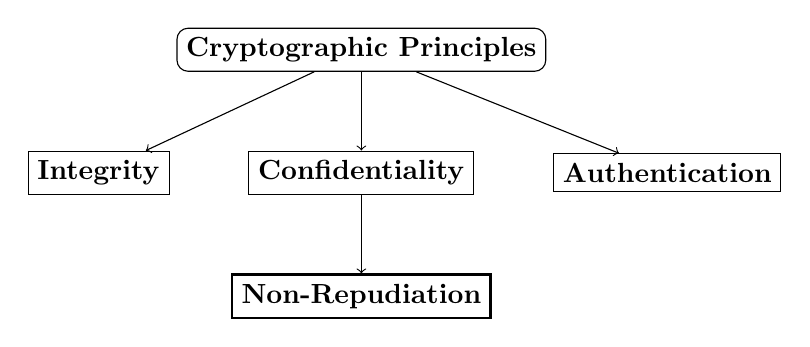
\begin{tikzpicture}
            \node (principles) [draw, rectangle, rounded corners] {\textbf{Cryptographic Principles}};
            \node (confidentiality) [draw, rectangle, below=of principles] {\textbf{Confidentiality}};
            \node (integrity) [draw, rectangle, left=of confidentiality] {\textbf{Integrity}};
            \node (authentication) [draw, rectangle, right=of confidentiality] {\textbf{Authentication}};
            \node (nonRepudiation) [draw, rectangle, below=of confidentiality, thick] {\textbf{Non-Repudiation}};
    
            \path[->] (principles) edge (confidentiality);
            \path[->] (principles) edge (integrity);
            \path[->] (principles) edge (authentication);
            \path[->] (confidentiality) edge (nonRepudiation);
        \end{tikzpicture}
    \end{center}
\end{frame}

\begin{frame}[fragile]
    \frametitle{Python Example: Hashing for Integrity}
    \begin{lstlisting}[language=Python]
import hashlib

# Function to create a hash
def create_hash(data):
    return hashlib.sha256(data.encode()).hexdigest()

# Example Usage
data = "Hello, World!"
hash_value = create_hash(data)
print(f"Hash: {hash_value}")
    \end{lstlisting}
\end{frame}

\begin{frame}
    \frametitle{Conclusion}
    The principles of confidentiality, integrity, authentication, and non-repudiation 
    are the backbone of secure cryptographic systems. 
    Understanding and applying them correctly is essential when implementing cryptography 
    in Python or any other programming language.
\end{frame}

\begin{frame}[fragile]
    \frametitle{Types of Cryptographic Algorithms - Overview}
    \begin{block}{Introduction}
        Cryptography is essential for securing information in digital communications. 
        In this slide, we will compare three primary categories of cryptographic algorithms:
        symmetric, asymmetric, and hash functions.
        Understanding these types is crucial for their effective application in real-world scenarios.
    \end{block}
\end{frame}

\begin{frame}[fragile]
    \frametitle{Types of Cryptographic Algorithms - Symmetric Cryptography}
    \begin{itemize}
        \item \textbf{Definition:} Uses the same key for both encryption and decryption.
        \item \textbf{How It Works:} 
        The sender and receiver share a secret key. 
        Data is encrypted using this key, and the same key is used for decryption.
    \end{itemize}

    \begin{block}{Example: Python Code}
    \begin{lstlisting}[language=Python]
from Crypto.Cipher import AES
import os

key = os.urandom(16)  # AES key (16 bytes for AES-128)
cipher = AES.new(key, AES.MODE_EAX)
ct, tag = cipher.encrypt_and_digest(b"Secret Message")
    \end{lstlisting}
    \end{block}

    \begin{itemize}
        \item \textbf{Use Cases:}
        \begin{itemize}
            \item Data encryption at rest (databases, file systems)
            \item Secure communications (VPNs)
            \item Bulk data encryption due to efficiency
        \end{itemize}
    \end{itemize}
\end{frame}

\begin{frame}[fragile]
    \frametitle{Types of Cryptographic Algorithms - Asymmetric Cryptography}
    \begin{itemize}
        \item \textbf{Definition:} 
        Uses a pair of keys: a public key for encryption and a private key for decryption.
        \item \textbf{How It Works:}
        The sender encrypts a message using the recipient's public key.
        Only the recipient can decrypt the message using their private key.
    \end{itemize}

    \begin{block}{Example: Python Code}
    \begin{lstlisting}[language=Python]
from Crypto.PublicKey import RSA
from Crypto.Cipher import PKCS1_OAEP

key = RSA.generate(2048)
public_key = key.publickey()
cipher = PKCS1_OAEP.new(public_key)
encrypted_message = cipher.encrypt(b"Hello, World!")
    \end{lstlisting}
    \end{block}

    \begin{itemize}
        \item \textbf{Use Cases:}
        \begin{itemize}
            \item Secure email (PGP)
            \item SSL/TLS for secure web browsing
            \item Digital signatures providing authentication and integrity
        \end{itemize}
    \end{itemize}
\end{frame}

\begin{frame}[fragile]
    \frametitle{Types of Cryptographic Algorithms - Hash Functions}
    \begin{itemize}
        \item \textbf{Definition:} 
        A one-way function that converts input data of any size into a fixed-size string of characters.
        \item \textbf{How It Works:}
        The output (hash) will always be the same for the same input but is infeasible to reverse-engineer.
    \end{itemize}

    \begin{block}{Example: Python Code}
    \begin{lstlisting}[language=Python]
import hashlib

message = b"Hello, World!"
hash_object = hashlib.sha256(message)
hash_digest = hash_object.hexdigest()
    \end{lstlisting}
    \end{block}

    \begin{itemize}
        \item \textbf{Use Cases:}
        \begin{itemize}
            \item Data integrity checks
            \item Password storage (salting and hashing)
            \item Digital signatures and blockchain technology
        \end{itemize}
    \end{itemize}
\end{frame}

\begin{frame}[fragile]
    \frametitle{Types of Cryptographic Algorithms - Key Points}
    \begin{itemize}
        \item \textbf{Symmetric Cryptography:} Fast but requires secure key exchange.
        \item \textbf{Asymmetric Cryptography:} Secures key exchange but is slower than symmetric encryption.
        \item \textbf{Hash Functions:} Essential for data integrity, not for encryption.
    \end{itemize}
\end{frame}

\begin{frame}[fragile]
    \frametitle{Types of Cryptographic Algorithms - Conclusion}
    \begin{block}{Conclusion}
        Understanding these three types of cryptographic algorithms—symmetric, asymmetric, and hash functions—is crucial for implementing robust security measures in applications. Each has distinct strengths and weaknesses, making them suitable for different scenarios in cybersecurity. 
    \end{block}

    \begin{block}{Key Takeaway}
        By mastering these concepts, you will be better equipped to apply cryptographic principles and choose the right algorithm for securing data in various contexts.
    \end{block}
\end{frame}

\begin{frame}[fragile]
    \frametitle{Cryptographic Protocols - Overview}
    \begin{block}{Understanding Cryptographic Protocols}
        Cryptographic protocols are standardized methods for secure communication. They utilize cryptographic algorithms and techniques to ensure data confidentiality, integrity, authenticity, and non-repudiation.
    \end{block}
    
    \begin{block}{Key Protocols}
        Some of the key cryptographic protocols include:
        \begin{enumerate}
            \item TLS/SSL
            \item IPsec
            \item PGP
        \end{enumerate}
    \end{block}
\end{frame}

\begin{frame}[fragile]
    \frametitle{Cryptographic Protocols - TLS/SSL and IPsec}
    
    \begin{block}{TLS (Transport Layer Security) / SSL (Secure Sockets Layer)}
        \begin{itemize}
            \item \textbf{Overview}: TLS is the successor to SSL, providing secure communication over a network.
            \item \textbf{Functionality}: Encrypts data between client and server.
            \item \textbf{Process}:
            \begin{itemize}
                \item Handshake: Establishes session keys.
                \item Authentication: Validates identity of parties.
                \item Data Encryption: Ensures data privacy.
            \end{itemize}
            \item \textbf{Example}: TLS encrypts your information on secure websites, e.g., online banking.
        \end{itemize}
    \end{block}

    \begin{block}{IPsec (Internet Protocol Security)}
        \begin{itemize}
            \item \textbf{Overview}: A suite of protocols to secure IP communication.
            \item \textbf{Applications}: Used in Virtual Private Networks (VPNs).
            \item \textbf{Operation}: Operates in Transport or Tunnel Mode to encrypt data.
            \item \textbf{Example}: Corporate VPNs using IPsec for secure remote access.
        \end{itemize}
    \end{block}
\end{frame}

\begin{frame}[fragile]
    \frametitle{Cryptographic Protocols - PGP and Key Points}
    
    \begin{block}{PGP (Pretty Good Privacy)}
        \begin{itemize}
            \item \textbf{Overview}: A program for securing emails using encryption.
            \item \textbf{Functionality}: Combines symmetric and asymmetric encryption.
            \item \textbf{Use Case}: Individuals and organizations use PGP for secure communication and data storage.
        \end{itemize}
    \end{block}

    \begin{block}{Key Points to Emphasize}
        \begin{itemize}
            \item \textbf{Importance of Secure Communication}: Protects sensitive data from interception.
            \item \textbf{Interoperability}: Works across various platforms and applications.
            \item \textbf{Continuous Evolution}: Adapts to evolving cyber threats.
        \end{itemize}
    \end{block}

    \begin{block}{Summary}
        Cryptographic protocols like TLS/SSL, IPsec, and PGP are vital for secure communications in our digital world.
    \end{block}
\end{frame}

\begin{frame}[fragile]
    \frametitle{Implementing Symmetric Cryptography in Python}
    \begin{itemize}
        \item Hands-on coding session covering Python libraries for symmetric encryption.
        \item Focus on data confidentiality through symmetric cryptography.
    \end{itemize}
\end{frame}

\begin{frame}[fragile]
    \frametitle{Overview of Symmetric Cryptography}
    \begin{block}{Definition}
        Symmetric cryptography uses the same key for both encryption and decryption.
    \end{block}
    
    \begin{itemize}
        \item \textbf{Key Characteristics:}
        \begin{itemize}
            \item Single Key Usage: Shared securely between sender and receiver.
            \item Speed: Generally faster than asymmetric methods.
            \item Common Algorithms: AES, DES, 3DES, RC4.
        \end{itemize}
    \end{itemize}
\end{frame}

\begin{frame}[fragile]
    \frametitle{Popular Python Libraries for Symmetric Encryption}
    \begin{enumerate}
        \item \textbf{Cryptography}: High-level interface for cryptographic functions.
        \item \textbf{PyCryptodome}: Self-contained Python package for low-level cryptography.
    \end{enumerate}
    
    \begin{block}{Example Implementation}
        \begin{lstlisting}[language=Python]
# Install the library if not already installed
# pip install cryptography

from cryptography.fernet import Fernet

# Generate a key
key = Fernet.generate_key()
cipher = Fernet(key)

# Encrypting a message
plaintext = b"My secret message"
ciphertext = cipher.encrypt(plaintext)
print("Ciphertext:", ciphertext)

# Decrypting the message
decrypted_text = cipher.decrypt(ciphertext)
print("Decrypted Text:", decrypted_text.decode())
        \end{lstlisting}
    \end{block}
\end{frame}

\begin{frame}[fragile]
    \frametitle{Explanation of Code}
    \begin{itemize}
        \item \textbf{Key Generation}: 
            \begin{itemize}
                \item \texttt{Fernet.generate\_key()} creates a secure key.
            \end{itemize}
        \item \textbf{Encryption}: 
            \begin{itemize}
                \item \texttt{cipher.encrypt()} takes a byte string and returns ciphertext.
            \end{itemize}
        \item \textbf{Decryption}: 
            \begin{itemize}
                \item \texttt{cipher.decrypt()} returns the original plaintext.
            \end{itemize}
    \end{itemize}
\end{frame}

\begin{frame}[fragile]
    \frametitle{Key Points and Conclusion}
    \begin{itemize}
        \item \textbf{Secure Key Management}: Store encryption keys securely and do not hard-code them.
        \item \textbf{Use of IV}: For algorithms that require an Initialization Vector (IV), follow best practices.
        \item \textbf{Library Documentation}: Check the 
        \href{https://cryptography.io/en/latest/}{Cryptography} and 
        \href{https://www.pycryptodome.org/src/introduction}{PyCryptodome} documentation for more features.
    \end{itemize}

    \begin{block}{Conclusion}
        Symmetric cryptography is vital for data protection. Python libraries facilitate easy implementation, ensuring confidentiality.
    \end{block}

    \textbf{Next Steps:} Prepare for the implementation of asymmetric cryptography using public key pairs.
\end{frame}

\begin{frame}
    \frametitle{Implementing Asymmetric Cryptography in Python}
    \begin{itemize}
        \item Practical coding session using Python libraries
        \item Focus on asymmetric cryptography concepts
        \item Hands-on example with key pair generation, encryption, and decryption
    \end{itemize}
\end{frame}

\begin{frame}
    \frametitle{Understanding Asymmetric Cryptography}
    \begin{block}{Key Concepts}
        \begin{itemize}
            \item \textbf{Public Key:} Used to encrypt data; can be shared publicly.
            \item \textbf{Private Key:} Used to decrypt data; must be kept secret.
        \end{itemize}
    \end{block}
    
    \begin{block}{Benefits}
        \begin{itemize}
            \item \textbf{Enhanced Security:} Public keys can be shared without compromising security.
            \item \textbf{Digital Signatures:} Ensures authenticity and integrity of messages.
        \end{itemize}
    \end{block}
\end{frame}

\begin{frame}[fragile]
    \frametitle{Implementing Asymmetric Cryptography in Python}
    \begin{block}{Installation}
        \begin{lstlisting}[language=bash]
pip install cryptography
        \end{lstlisting}
    \end{block}

    \begin{block}{Example Implementation}
        \begin{lstlisting}[language=Python]
from cryptography.hazmat.backends import default_backend
from cryptography.hazmat.primitives.asymmetric import rsa, padding
from cryptography.hazmat.primitives import serialization, hashes

# 1. Generate a key pair
private_key = rsa.generate_private_key(
    public_exponent=65537,
    key_size=2048,
    backend=default_backend()
)

public_key = private_key.public_key()

# 2. Serialize the public key
pem = public_key.public_bytes(
    encoding=serialization.Encoding.PEM,
    format=serialization.PublicFormat.SubjectPublicKeyInfo
)

# 3. Encrypt a message
message = b'Secure message'
ciphertext = public_key.encrypt(
    message,
    padding.OAEP(
        mgf=padding.MGF1(algorithm=hashes.SHA256()),
        algorithm=hashes.SHA256(),
        label=None
    )
)

# 4. Decrypt the message
plaintext = private_key.decrypt(
    ciphertext,
    padding.OAEP(
        mgf=padding.MGF1(algorithm=hashes.SHA256()),
        algorithm=hashes.SHA256(),
        label=None
    )
)

print("Original message:", message)
print("Ciphertext:", ciphertext)
print("Decrypted message:", plaintext)
        \end{lstlisting}
    \end{block}
\end{frame}

\begin{frame}
    \frametitle{Important Points to Consider}
    \begin{itemize}
        \item Ensure that the private key is securely stored and never exposed.
        \item Choose between RSA or Elliptic Curve Cryptography (ECC) based on your needs.
        \item Always use secure padding (like OAEP) when encrypting data.
    \end{itemize}
\end{frame}

\begin{frame}
    \frametitle{Summary}
    \begin{itemize}
        \item Explored basics of asymmetric cryptography.
        \item Implemented key pair generation, encryption, and decryption in Python.
        \item Emphasized importance of keeping the private key confidential.
    \end{itemize}
\end{frame}

\begin{frame}
    \frametitle{Prepare for Next Slide}
    \begin{itemize}
        \item Next topic: \textbf{Risk Assessment in Cryptography}
        \item Focus on identifying vulnerabilities and potential attack vectors.
    \end{itemize}
\end{frame}

\begin{frame}
    \frametitle{Risk Assessment in Cryptography}
    \begin{block}{Overview}
        Effective cryptographic implementations are paramount to ensure the confidentiality, integrity, and authenticity of information. Understanding and managing risks is crucial to mitigate vulnerabilities and protect cryptographic systems from potential attacks.
    \end{block}
\end{frame}

\begin{frame}
    \frametitle{Key Concepts}
    \begin{enumerate}
        \item \textbf{Vulnerabilities}:
        \begin{itemize}
            \item Weaknesses in a system that can be exploited by attackers.
            \item Examples include:
            \begin{itemize}
                \item Broken algorithms (e.g., outdated hash functions like MD5).
                \item Poor key management practices (e.g., hardcoded keys in code).
                \item Flaws in implementation (e.g., buffer overflows).
            \end{itemize}
        \end{itemize}

        \item \textbf{Attack Vectors}:
        \begin{itemize}
            \item Paths through which an attack can occur.
            \item Common attack vectors include:
            \begin{itemize}
                \item \textbf{Man-in-the-Middle (MitM)}: Intercepting communication between two parties.
                \item \textbf{Replay Attacks}: Resending valid data transmission to deceive the recipient.
                \item \textbf{Side-channel Attacks}: Exploiting information gained from the physical implementation (e.g., timing attacks).
            \end{itemize}
        \end{itemize}
    \end{enumerate}
\end{frame}

\begin{frame}
    \frametitle{Risk Management Practices}
    \begin{enumerate}
        \item \textbf{Identify and Evaluate Risks}:
        \begin{itemize}
            \item Conduct regular security assessments, including penetration testing.
            \item Use tools to identify vulnerabilities (e.g., OWASP ZAP for web applications).
        \end{itemize}
        
        \item \textbf{Implement Best Practices}:
        \begin{itemize}
            \item Use up-to-date cryptographic algorithms and libraries (e.g., PyCryptodome in Python).
            \item Ensure proper key lifecycle management: generation, storage, rotation, and destruction.
        \end{itemize}
        
        \item \textbf{Continuous Monitoring}:
        \begin{itemize}
            \item Regularly check for vulnerabilities due to emerging threats (stay informed with CVE lists).
            \item Monitor system logs for suspicious activities.
        \end{itemize}
        
        \item \textbf{Documentation and Policies}:
        \begin{itemize}
            \item Maintain clear documentation of cryptographic protocols and policies.
            \item Train personnel on security best practices to create a culture of security awareness.
        \end{itemize}
    \end{enumerate}
\end{frame}

\begin{frame}[fragile]
    \frametitle{Example: Secure Key Generation in Python}
    \begin{lstlisting}[language=Python]
from Cryptodome.PublicKey import RSA

# Generate a secure RSA key pair
key = RSA.generate(2048)
private_key = key.export_key()
public_key = key.publickey().export_key()

# Securely store the keys, do NOT hardcode in production code
with open('private_key.pem', 'wb') as f:
    f.write(private_key)

with open('public_key.pem', 'wb') as f:
    f.write(public_key)
    \end{lstlisting}
\end{frame}

\begin{frame}
    \frametitle{Key Points to Emphasize}
    \begin{itemize}
        \item \textbf{Proactive Risk Assessment}: Regularly identifying vulnerabilities is better than reactive measures.
        \item \textbf{Adopting Best Practices}: Following industry-standard practices can significantly reduce security risks.
        \item \textbf{Stay Informed}: The landscape of cryptography evolves, and continuous learning is essential.
    \end{itemize}
\end{frame}

\begin{frame}[fragile]
    \frametitle{Emerging Technologies in Cryptography - Overview of Trends}
    
    \begin{itemize}
        \item \textbf{Quantum Cryptography:} Uses quantum mechanics for secure communication.
        \begin{itemize}
            \item Relies on physical principles rather than algorithms.
            \item \textbf{Key Mechanism:} Quantum Key Distribution (QKD) using photon polarization.
        \end{itemize}
        
        \item \textbf{Blockchain Technology:} A decentralized digital ledger for secure transactions.
        \begin{itemize}
            \item \textbf{Key Features:} Decentralization and cryptographic hashing.
        \end{itemize}
    \end{itemize}
\end{frame}

\begin{frame}[fragile]
    \frametitle{Emerging Technologies in Cryptography - Key Implications}
    
    \begin{block}{Quantum Cryptography}
        \begin{itemize}
            \item Generates keys invulnerable to eavesdropping.
            \item Adoption challenges include distance limitations and hardware requirements.
        \end{itemize}
    \end{block}
    
    \begin{block}{Blockchain Technology}
        \begin{itemize}
            \item Ensures data integrity and immutability.
            \item Enables smart contracts for programmable transactions.
        \end{itemize}
    \end{block}
\end{frame}

\begin{frame}[fragile]
    \frametitle{Emerging Technologies in Cryptography - Examples and Conclusion}

    \begin{itemize}
        \item \textbf{Examples:}
        \begin{itemize}
            \item \textbf{QKD Implementation:} China's quantum satellite for long-distance communication.
            \item \textbf{Blockchain Example:} Bitcoin's secure transaction framework.
        \end{itemize}

        \item \textbf{Conclusion:} 
        The integration of quantum mechanics and blockchain is transforming secure communications. Understanding these technologies is crucial for cybersecurity and data protection fields.
    \end{itemize}
\end{frame}

\begin{frame}[fragile]
    \frametitle{Emerging Technologies in Cryptography - Code Example}

    \begin{lstlisting}[language=Python]
import hashlib

def create_block(data, previous_hash):
    block_content = str(data) + str(previous_hash)
    block_hash = hashlib.sha256(block_content.encode()).hexdigest()
    return block_hash

# Example usage
previous_hash = '0000000000000000000'
data = {'transaction': 'Alice pays Bob 5 BTC'}
new_block_hash = create_block(data, previous_hash)
print("New Block Hash:", new_block_hash)
    \end{lstlisting}
    
    \begin{itemize}
        \item This code demonstrates how a hash is generated for a new block in a blockchain by combining its data with the previous block's hash.
    \end{itemize}
\end{frame}

\begin{frame}[fragile]
    \frametitle{Ethical and Legal Considerations - Introduction}
    \begin{block}{Introduction to Cryptography Ethics}
        Cryptography is a powerful tool used to protect information and ensure privacy, but its use raises significant ethical and legal issues. Understanding these considerations is essential for practitioners in the field of computer science and cybersecurity.
    \end{block}
\end{frame}

\begin{frame}[fragile]
    \frametitle{Ethical Considerations}
    \begin{enumerate}
        \item \textbf{Privacy vs. Security}
            \begin{itemize}
                \item Dilemma: Cryptography secures personal information but may hide illegal activities.
                \item Example: Encrypted communication apps can protect activists but may also be misused by criminals.
            \end{itemize}

        \item \textbf{Responsible Use}
            \begin{itemize}
                \item Ethical use promotes transparency and accountability.
                \item Developers should consider potential misuse scenarios.
            \end{itemize}

        \item \textbf{Access to Information}
            \begin{itemize}
                \item Should governments access encrypted communications for security? 
                \item Example: The "going dark" debate, where law enforcement struggles with encrypted communications.
            \end{itemize}
    \end{enumerate}
\end{frame}

\begin{frame}[fragile]
    \frametitle{Legal Frameworks}
    \begin{enumerate}
        \item \textbf{Data Privacy Laws}
            \begin{itemize}
                \item Regulations such as GDPR emphasize the importance of data encryption.
                \item Key point: Non-compliance can result in heavy fines and legal actions.
            \end{itemize}

        \item \textbf{Export Laws}
            \begin{itemize}
                \item Strict regulations on cryptographic technology export, impacting national security.
                \item Example: U.S. licensing rules restrict distribution to certain countries.
            \end{itemize}

        \item \textbf{Legislation on Encryption}
            \begin{itemize}
                \item Some laws mandate corporate backdoors to encrypted data.
                \item Example: The UK’s Investigatory Powers Act allows government access to data.
            \end{itemize}
    \end{enumerate}
\end{frame}

\begin{frame}[fragile]
    \frametitle{Key Points and Conclusion}
    \begin{block}{Key Points}
        \begin{itemize}
            \item Balance between Privacy and Security
            \item Legal Consequences of non-compliance
            \item Ethical Responsibility in programming
        \end{itemize}
    \end{block}
    
    \begin{block}{Conclusion}
        Ethical and legal considerations are paramount in cryptographic systems. Awareness enables developers to create socially responsible and compliant systems.
    \end{block}
\end{frame}

\begin{frame}[fragile]
    \frametitle{Example Code Snippet}
    \begin{lstlisting}[language=Python]
from cryptography.fernet import Fernet

# Generate key
key = Fernet.generate_key()
cipher_suite = Fernet(key)

# Encrypting a message
plaintext = b"Secret Message"
ciphertext = cipher_suite.encrypt(plaintext)
print("Encrypted:", ciphertext)

# Decrypting the message
decrypted_message = cipher_suite.decrypt(ciphertext)
print("Decrypted:", decrypted_message.decode())
    \end{lstlisting}
    
    \begin{block}{Note}
        Always consider ethical implications when deciding to encrypt sensitive information and adhere to legal regulations surrounding cryptographic technologies.
    \end{block}
\end{frame}


\end{document}